\subsection*{Геометрия, тернарный поиск [10]}
\begin{center}
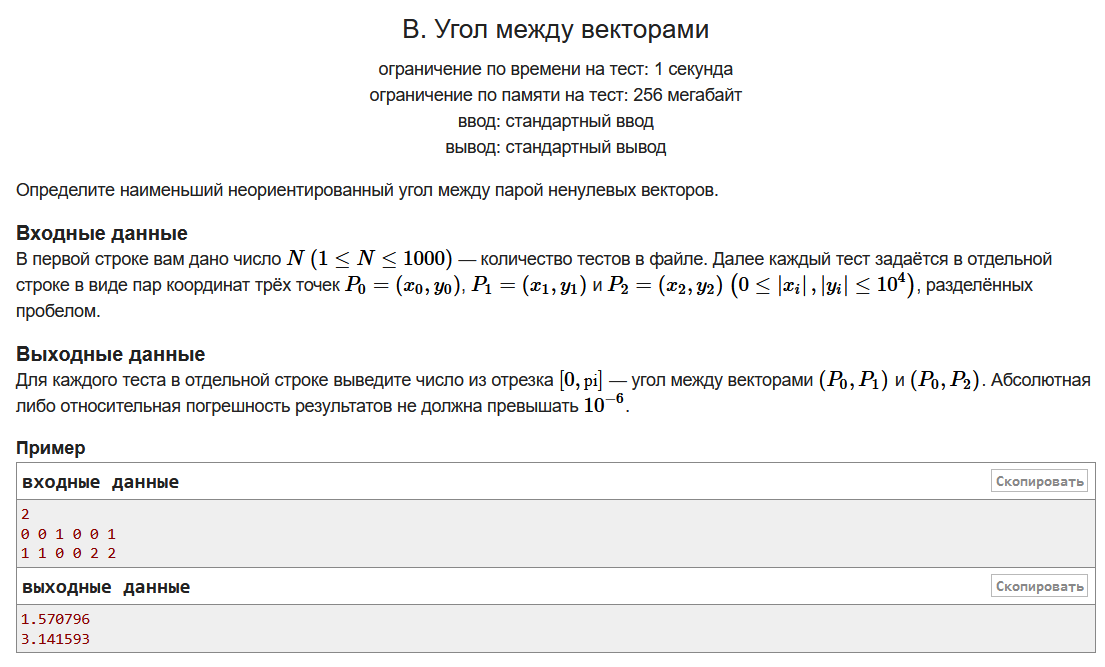
\includegraphics[width=\textwidth]{12B.png}
\end{center}
\subsubsection*{Идея решения}
Реализуем векторы и операции над ними. Угол между двумя векторами находится с помощью функции взятия арктангенса между векторным произведением и скалярным произведением, но здесь угол имеет диапазон от [$-2\pi; 2\pi$], а в условии сказано найти от $[0; \pi]$, поэтому возьмем модуль от полученного угла. 
\subsubsection*{Исходный код}
\begin{lstlisting}
#include <iostream>
#include <sstream>
#include <fstream>
#include <iomanip>
#include <string>
#include <cstdlib>
#include <cstdio>
#include <cstring>
#include <cmath>
#include <ctime>
#include <climits>
#include <cassert>
#include <vector>
#include <queue>
#include <stack>
#include <deque>
#include <set>
#include <map>
#include <bitset>
#include <utility>
#include <algorithm>
#include <unordered_map>
using namespace std;

const double eps = 10e-3;
struct point {
    double x, y;
    point() {}
    point(double a, double b) : x(a), y(b) {}
};

point operator -(const point& a, const point& b) {
    return point(a.x - b.x, a.y - b.y);
}

double scal(point a, point b) {
    return a.x * b.x + a.y * b.y;
}

double vec(point a, point b) {
    return a.x * b.y - b.x * a.y;
}

double ug(point a, point b) {
    return(atan2(vec(a, b), scal(a, b)));
}

double len(const point a, const point b) {
    return (sqrt((b.x - a.x) * (b.x - a.x) + (b.y - a.y) * (b.y - a.y)));
}

istream& operator >>(istream& in, point& p) {
    in >> p.x >> p.y;
    return in;
}

bool eql(double a, double b) {
    if (abs(a - b) < eps) {
        return true;
    }
    return false;
}

int main() {
    ios_base::sync_with_stdio(false);
    cin.tie(0);
    cout.tie(0);
    int n;
    cin >> n;
    for (int i = 0; i < n; i++) {
        point a, b;
        int x0, y0, x1, y1, x2, y2;
        cin >> x0 >> y0 >> x1 >> y1 >> x2 >> y2;
        a = point(x1 - x0, y1 - y0);
        b = point(x2 - x0, y2 - y0);
        cout << fixed << setprecision(6) << abs(ug(a, b)) << '\n';
    }
    return 0;
}
\end{lstlisting}
\subsubsection*{Фрагмент турнирной таблицы контеста}
\begin{center}
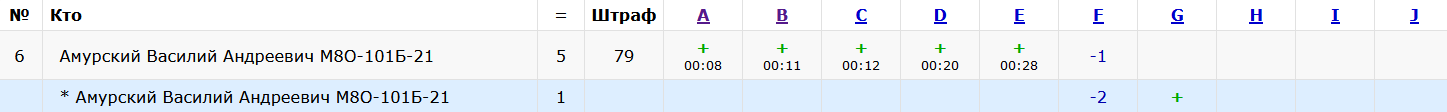
\includegraphics[width=\textwidth]{state12.png}\newline\noindent
\end{center}

\subsubsection*{Выводы}
Задача решена, проблем не возникло.
